\section{Unsupervised approaches} 
\label{section:rel-unsupervised} 

Unsupervised methods eliminate the need for ground-truth data, which typically requires time-consuming and labor-intensive manual annotation. Instead, unsupervised approaches leverage large collections of original videos for training. Through learning mechanisms designed for unsupervised settings, these methods extract meaningful information from the video data to generate summaries.

\subsection{Fooling Discriminator to Discriminate Original Video from Summary-Based Reconstruction}
\label{section:rel-unsup-discriminative}

\begin{figure}[ht]
    \centering
    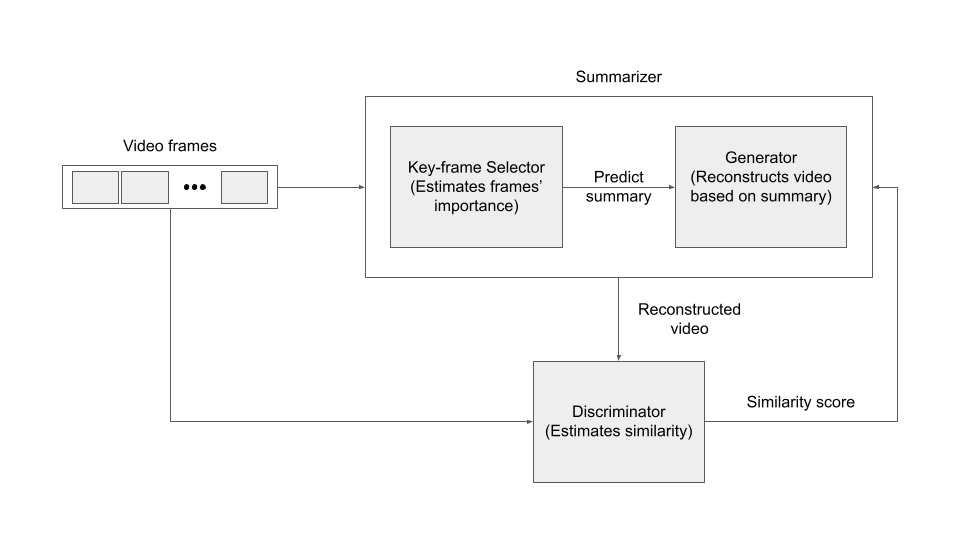
\includegraphics[width=0.73\paperwidth]{content/related/figures/unsup-gan.png}
    \caption{High-level representation of the analysis pipeline of unsupervised
    algorithms that learn summarization by increasing the similarity between the
    summary and the video.}
    \label{figure:rel-unsup-gan}
  \end{figure}

To address the absence of ground-truth data, unsupervised techniques leverage the principle that a representative summary should enable viewers to comprehend the original video content. To achieve this, Generative Adversarial Networks (GANs) are employed to learn the creation of video summaries that facilitate accurate reconstruction of the original video. The training process (see \hyperref[figure:rel-unsup-gan]{Figure \ref{figure:rel-unsup-gan}}) involves a Summarizer, consisting of a Key-frame Selector and a Generator. The Key-frame Selector estimates frame importance and generates a summary, while the Generator reconstructs the video based on the generated summary. By inputting the video frames and predicting frame-level importance scores, the Summarizer reconstructs the original video. The reconstructed video, alongside the original one, is fed into a trainable Discriminator that evaluates their similarity. Similar to supervised GAN-based methods, the training of the entire summarization architecture follows an adversarial approach. In this case, the Summarizer's objective is to deceive the Discriminator by making it challenging to distinguish between the summary-based reconstructed video and the original video. Conversely, the Discriminator aims to improve its discrimination abilities. When the discrimination becomes indistinguishable (i.e., similar classification error for both videos), the Summarizer successfully constructs a highly representative video summary.  

Notably, Mahasseni \etal~\cite{mahasseni2017unsupervised} combined an LSTM-based key-frame selector, a Variational Auto-Encoder (VAE), and a trainable Discriminator, using adversarial learning to minimize the distance between the original video and the summary-based reconstructed version. Building upon this foundation, Apostolidis \etal~\cite{apostolidis2019stepwise} proposed a stepwise, label-based approach for training the adversarial part of the network, leading to enhanced summarization performance. Yuan \etal~\cite{yuan2019cycle} introduced an approach aiming to maximize the mutual information between the summary and the video, utilizing a pair of trainable discriminators and a cycle-consistent adversarial learning objective. Their frame selector, a bidirectional LSTM, constructs a video summary by modeling temporal dependencies among frames. The summary is then evaluated by two GANs—an encoder-decoder GAN for forward reconstruction and a backward GAN for reverse reconstruction. The consistency between these reconstructions quantifies information preservation, guiding the frame selector to identify the most informative frames for the video summary. In a subsequent work, Apostolidis \etal~cite{apostolidis2020ac} integrated an Actor-Critic model into a GAN, formulating the selection of important video fragments as a sequence generation task. The Actor and Critic engage in a game that incrementally selects video key fragments, with rewards from the Discriminator influencing their choices. This training workflow enables the Actor and Critic to learn a value function (Critic) and a policy for key-fragment selection (Actor). Other approaches extended the core VAE-GAN architecture by incorporating tailored attention mechanisms. For instance, Jung \etal~\cite{jung2019discriminative} proposed a VAE-GAN architecture extended with a chunk and stride network (CSNet) and a tailored difference attention mechanism, capturing frame dependencies at various temporal granularities during keyframe selection. In a subsequent work, Jung \etal~\cite{jung2020global} introduced a self-attention mechanism combined with relative position modeling, decomposing the frame sequence into non-overlapping groups to capture both local and global interdependencies. Apostolidis \etal~\cite{apostolidis2020unsupervised} presented a variation of their prior work \cite{apostolidis2019stepwise}, replacing the VAE with a deterministic Attention Auto-Encoder to improve attention-driven reconstruction and key-fragment selection. He \etal~\cite{he2019unsupervised} proposed a self-attention-based conditional GAN, utilizing a conditional feature selector and a multi-head self-attention mechanism to focus on important temporal regions and model long-range dependencies in the video sequence. Finally, Rochan \etal~\cite{rochan2019video} developed an approach for video summarization from unpaired data, employing an adversarial process with GANs and a Fully-Convolutional Sequence Network (FCSN) encoder-decoder. The model aimed to learn a mapping function from raw video to a human-like summary, aligning the summary distribution with human-created summaries while ensuring content diversity through an applied constraint on the learned mapping function.

These techniques aim to generate representative video summaries by fooling the Discriminator, making it difficult to distinguish between the summary-based reconstruction and the original video. By achieving similar classification errors for both, it indicates that the Summarizer has successfully created a summary that captures the overall video content.

\subsection{Focusing on Specific Desired Properties}
\label{subsec:rel-unsup-specific-properties}

% Addressing the challenges of unstable training and limited evaluation criteria in GAN-based methods, certain unsupervised approaches focus on specific properties of an optimal video summary. These approaches employ reinforcement learning principles in conjunction with hand-crafted reward functions that quantify desired characteristics in the generated summary. Illustrated in Fig. 6, the Summarizer takes the video frame sequence as input and generates a summary by predicting frame-level importance scores. The predicted summary is then evaluated by an Evaluator, which employs hand-crafted reward functions to measure the presence of specific desired characteristics. The computed scores are combined to form an overall reward value, guiding the training of the Summarizer.

% The initial work in this direction, proposed by Zhou et al. (2018), formulates video summarization as a sequential decision-making process. They train a Summarizer to produce diverse and representative video summaries using a diversity-representativeness reward. The diversity reward quantifies the dissimilarity among selected keyframes, while the representativeness reward measures the visual resemblance of the selected keyframes to the remaining frames of the video.

% Expanding on this method, Yaliniz et al. (2021) present another reinforcement-learning-based approach that incorporates the uniformity of the generated summary. They employ Independently Recurrent Neural Networks (IndRNNs) activated by a Leaky ReLU function to model temporal dependencies among frames. This addresses issues related to decaying, vanishing, and exploding gradients in LSTM models and facilitates better learning of long-term dependencies. In addition to rewards associated with representativeness and diversity, Yaliniz et al. introduce a uniformity reward to enhance the coherence of the summary and prevent redundant jumps between selected video fragments.

% Gonuguntla et al. (2019) propose a method utilizing Temporal Segment Networks, originally designed for action recognition in videos, to extract spatial and temporal information from video frames. They train the Summarizer using a reward function that evaluates the preservation of the video's main spatiotemporal patterns in the generated summary.

% Lastly, Zhao et al. (2020) present a mechanism that combines video summarization and reconstruction. Video reconstruction aims to estimate how well the summary allows viewers to infer the original video, similar to some GAN-based methods. Video summarization is learned based on feedback from the reconstructor and the output of trained models that assess the representativeness and diversity of the visual content in the generated summary.


\subsection{Building Object-Oriented Summaries through Key Object Motion}
\label{subsec:rel-unsup-object-oriented}

Zhang \etal~\cite{zhang2020unsupervised} devised a novel method that prioritizes the retention of fine-grained semantic and motion details within the video summary. Their approach involves an initial preprocessing step aimed at identifying significant objects and their key motions. Leveraging this information, the method represents the entire video by creating segmented object motion clips. Subsequently, these clips are fed into the Summarizer, which employs an online motion auto-encoder model known as Stacked Sparse LSTM Auto-Encoder. This model continually updates a customized recurrent auto-encoder network to encode and memorize previous states of object motions. The network's primary task is to reconstruct object-level motion clips, with the reconstruction loss computed between the input and output frames serving as a guide for training the Summarizer. Through this training process, the Summarizer becomes proficient in generating summaries that highlight the representative objects in the video and the key motions associated with each object.

